% p41-operator-p-representable-over-a-cpo.tex
%
% Source: Carl A. Gunter and Dana S. Scott, "Semantic Domains".
%   physical page 41 of ScottDomains/papers/Gunter Scott 1990.pdf
%   printed page 40
%   section 7.3, "Solving domain equations with projections."
%   unnamed in the paper; introduced by this sentence:
%
%   "Let us say that an operator F on cpo's is p-representable over a cpo U if
%    and only if there is a continuous function R_F which completes the
%    following diagram (up to isomorphism):"
%
%   followed by "Since there will be no chance of confusion, let us just use
%   the term 'representable' for 'p-representable' for the remainder of this
%   section."
%
% What the diagram says: the same universal property as the page 35 diagram,
% with finitary *projections* in place of finitary closures.  Fp(U) replaces
% Fc(U); everything else is identical, which is the point — section 7.3 redoes
% section 7.1's construction with projections because PN cannot represent the
% sum operator +.  Solid arrows are the given maps (the operator F, and im);
% the dashed R_F is the map asserted to exist.  Keep the distinction.
%
% The development uses this to reach Theorem 27 (a projection p : U -> D for
% every bounded complete domain D) and Lemma 28's operator list, and then
% section 7.4 repeats the pattern once more over V for the bifinites, where
% Lemma 30 adds the convex powerdomain.
%
% Geometry: measured from the page.  A 300 dpi crop of the region (candidate
% row "41 620 773 101 734" of the r0039 candidate log) puts the square at
% 474 x 237 px, i.e. 113.8 x 56.9 pt — the same macro as page 35's diagram — so
% 4 cm x 2 cm reproduces the paper's own size at 28.45 pt per cm.

\documentclass[border=6pt]{standalone}
\usepackage{tikz}
\begin{document}
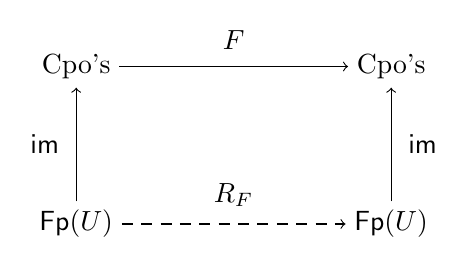
\begin{tikzpicture}[
  x=1cm, y=1cm,
  every node/.style={inner sep=1pt},
  open/.style={circle, draw, fill=white, minimum size=4pt, inner sep=0pt},
  solid/.style={circle, draw, fill=black, minimum size=5pt, inner sep=0pt},
  edge/.style={draw, line width=0.4pt},
  obj/.style={inner sep=3pt},
  arrow/.style={draw, line width=0.4pt, ->},
  darrow/.style={draw, line width=0.4pt, ->, dash pattern=on 4pt off 3pt}]

  % ---- objects ------------------------------------------------------------
  \node[obj] (TL) at (0,2) {Cpo's};
  \node[obj] (TR) at (4,2) {Cpo's};
  \node[obj] (BL) at (0,0) {$\mathsf{Fp}(U)$};
  \node[obj] (BR) at (4,0) {$\mathsf{Fp}(U)$};

  % ---- arrows -------------------------------------------------------------
  % label offsets are the paper's: 11 pt clear of the arrow, measured off a
  % 300 dpi crop (4.167 px/pt) as 46-48 px from label centre to arrow.
  \draw[arrow]  (TL) -- node[above=5pt] {$F$}   (TR);
  \draw[darrow] (BL) -- node[above=5pt] {$R_F$} (BR);
  \draw[arrow]  (BL) -- node[left=5pt]  {$\mathsf{im}$} (TL);
  \draw[arrow]  (BR) -- node[right=5pt] {$\mathsf{im}$} (TR);
\end{tikzpicture}
\end{document}
